\documentclass[11pt]{article}
\usepackage{tikz}
\usetikzlibrary{calc}
\usepackage{eso-pic}
\usepackage{lipsum}
\usepackage{xcolor}
\usepackage{listings}
\usepackage{gensymb}
\usepackage[english]{babel}
\usepackage[utf8x]{inputenc}
\usepackage{amsmath}
\usepackage{graphicx}
\usepackage[colorinlistoftodos]{todonotes}
\usepackage{enumitem}
\usepackage{listings}
\usepackage{filecontents}
\usepackage{verbatim}
\usepackage{eurosym}
\usepackage[export]{adjustbox}
\usepackage{hyperref}
\usepackage{textcomp}
\usepackage{tabularx}
\usepackage{hyperref}
\usepackage{xurl}
\usepackage{float}
\usepackage{xepersian}
\settextfont{Niloofar.ttf}
\renewcommand{\baselinestretch}{1.5}

\AddToShipoutPictureBG{%
\begin{tikzpicture}[overlay,remember picture]
\draw[line width=4pt]
    ($ (current page.north west) + (1cm,-1cm) $)
    rectangle
    ($ (current page.south east) + (-1cm,1cm) $);
\draw[line width=1.5pt]
    ($ (current page.north west) + (1.2cm,-1.2cm) $)
    rectangle
    ($ (current page.south east) + (-1.2cm,1.2cm) $);
\end{tikzpicture}
}

\begin{document}

\begin{titlepage}

\newcommand{\HRule}{\rule{\linewidth}{0.5mm}}

\center 

\textsc{\LARGE به نام خدا}\\[1cm] 


\includegraphics[width=0.4\textwidth]{Images/IUSTLogo.png}\\[1cm] 

\textsc{\Large درس امنیت سیستم های کامپیوتری  }

\HRule \\[0.4cm]
{ \huge \bfseries تمرین سری دوم فصل دو(پرومتیم) }\\ 
\HRule \\[1.5cm]

\begin{minipage}{0.4\textwidth}
\begin{center} \large
\emph{مدرس درس: } \\
جناب آقای دکتر دیانت \\[1cm]
\emph{تهیه شده توسط: }\\
فرزان رحمانی، \\
محمدحسین عباسپور
\end{center}
\end{minipage}\\[1cm]
{\large تاریخ ارسال: 1403/01/30}\\[2cm]
\vfill 

\end{titlepage}
\section*{\textcolor{orange}{سوال 1:}}
پیاده‌‌سازی یک روش نهان‌کاوی به عنوان آشکارسازی بر نهان‌نگاری به روش \lr{LSB} .یعنی فرض کنید که ما با روش \lr{LSB} عملیات نهان‌نگاری را انجام دادیم، شما باید یک روش نهان‌کاوی به منظور تشخیص آن پیاده‌سازی کنید.
\subsection*{\textcolor{cyan}{پاسخ 1:}}
کد موردنظر برای این بخش را در فایل \lr{Q1.ipynb} پیاده‌سازی کردیم. برای اینکه یک تصویر داشته باشیم تا بتوانیم عملیات نهان‌کاوی را روی آن انجام دهیم، در کدمان یک بخش برای \lr{encode} کردن تصویر، و یک بخش برای \lr{decode} آن قرار دادیم. سپس تصویر موردنظر را با پیام دلخواه \lr{encode} کردیم. همانطور که می‌دانیم در این روش برای \lr{encode} کردن تصویر، پیام در بیت‌های \lr{LSB} پیکسل‌ها قرار می‌گیرند؛ چرا که این بیت‌ها کم‌ارزش‌ترین بیت‌ها هستند و تغییر در آن‌ها، تفاوت چندانی در تصویر ایجاد نمی‌کند. در تابع \lr{Encode}، این اتفاق می‌افتد.
\begin{figure}[H]
  \centering
  
\includegraphics[width=0.65\textwidth]{Images/farzan.png}
  \caption{تصویر اصلی قبل از عملیات \lr{encoding}}   
\end{figure}
حال پس از انتخاب تصویر موردنظر برای عملیات نهان‌کاوی، برنامه را \lr{run} کرده و گزینه \lr{encode} را انتخاب می‌کنیم تا تصویر رمزگذاری شده برای مرحله بعد را آماده نماییم. همچنین کلمه \lr{Security} را به عنوان پیام پنهان به برنامه می‌دهیم. در انتها نیز آدرس مقصد برای ذخیره عکس \lr{encode} شده را می‌دهیم.
\begin{figure}[H]
  \centering
  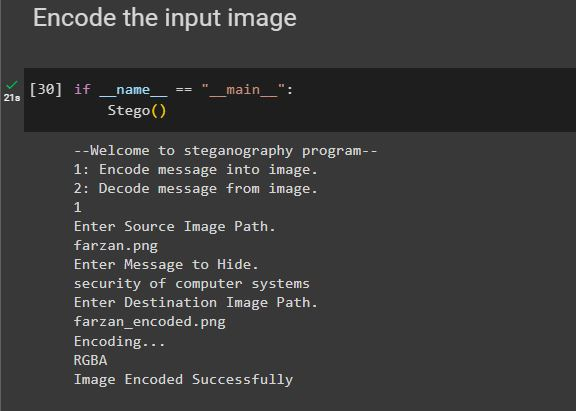
\includegraphics[width=0.7\textwidth]{Images/q1_1.JPG}
  \caption{نحوه \lr{encode} کردن تصویر}   
\end{figure}
حال تصویر رمزنگاری شده را بررسی می‌کنیم. همانطور که در شکل زیر نیز می‌بینید، تصویر رمزنگاری شده تفاوت چندانی با تصویر اصلی ندارد؛ به‌گونه‌ای که تغییرات با چشم غیرمسلح قابل مشاهده نیست. یکی از دلایل این پدیده می‌تواند کوتاه بودن متن پیام باشد. عبارت \lr{\$t3g0} به کار رفته هنگام ذخیره‌سازی تصویر نیز برای تشخیص انتهای پیام می‌باشد.
\begin{figure}[H]
  \centering
  
\includegraphics[width=0.5\textwidth]{Images/farzan_encoded.png}
  \caption{تصویر \lr{encode} شده}   
\end{figure}
حال از تابع \lr{Decode} برای نهان‌کاوی تصویر \lr{encode} شده استفاده می‌نماییم. همانطور که در شکل زیر مشاهده می‌نمایید، برنامه به‌درستی کلمه \lr{Security} که به عنوان پیام پنهان به تابع \lr{Encode} داده بودیم را برای ما چاپ می‌کند.
\begin{figure}[H]
  \centering
  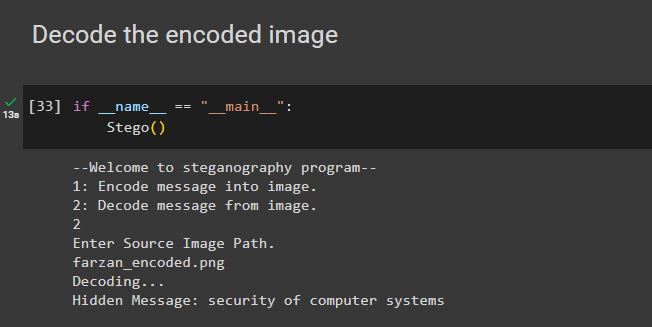
\includegraphics[width=0.6\textwidth]{Images/q1_2.JPG}
  \caption{نحوه \lr{decode} کردن تصویر}   
\end{figure}
\begin{latin}
\href{https://medium.com/swlh/lsb-image-steganography-using-python-2bbbee2c69a2}{\textcolor{blue}{Reference}}
\end{latin}
\section*{\textcolor{orange}{سوال 2:}}
پیاده سازی یک روش نشان گذاری. پیاده سازی باید به زبان های \lr{C++} یا \lr{Python} باشد.
\subsection*{\textcolor{cyan}{پاسخ 2:}}
نشان گذاری(watermarking) فرآیند جاسازی یک سیگنال دیجیتال منحصر به فرد و قابل شناسایی است که به عنوان واترمارک شناخته می‌ شود. واترمارکینگ در یک شی‌ چندرسانه ای مانند تصویر، ویدئو یا فایل صوتی‌ واترمارک می‌ تواند برای تأیید صحت یا مالکیت شی‌ یا برای ردیابی توزیع و استفاده از آن استفاده شود. واترمارک ها اغلب به گونه ای طراحی‌ می‌ شوند که برای چشم یا گوش انسان نامحسوس باشند تا در کیفیت یا محتوای رسانه تداخلی‌ ایجاد نکنند. تکنیک های مختلفی‌ برای واترمارک وجود دارد، از جمله واترمارک های قابل مشاهده و غیر قابل مشاهده و واترمارک های شکننده و غیرشکننده.

ما برای این پیاده سازی این تمرین از روش نشان گذاری(واترماکینگ) از نوع قابل مشاهده و غیرشکننده استفاده کزدیم. 

\textbf{واترمارک قابل مشاهده}: نمونه ای از واترمارک قابل مشاهده زمانی‌ است که یک عکاس آرم یا اطلاعات حق چاپ خود را به یک تصویر اضافه می‌ کند. این باعث می‌ شود که تصویر متعلق به آنها باشد و بدون اجازه نمی‌ توان از آن استفاده کرد.

\textbf{واترمارک غیرشکننده}: واترمارک غیرشکننده نوعی‌ از واترمارک است که در آن واترمارک همچنان قابل تشخیص است حتی‌ اگر رسانه به نحوی تغییر کرده باشد. به عنوان مثال، اگر هنرمندی بخواهد از موسیقی‌ خود در برابر دزدی محافظت کند، می‌ تواند یک واترمارک قوی در فایل صوتی‌ جاسازی کند. حتی‌ اگر کسی‌ سعی‌ کند فایل را با تغییر میزان بیت، فرمت یا طول تغییر دهد، واترمارک همچنان قابل تشخیص است. این باعث می‌ شود که برای ردیابی توزیع رسانه های دارای حق چاپ مفید باشد. هدف از واترمارک غیرشکننده این است که اطمینان حاصل شود که حتی‌ اگر رسانه به نحوی تغییر کرده باشد، مانند فشردە سازی، برش، تغییر اندازه، چرخش، اضافه کردن نویز هنوز واترمارک قابل شناسایی است.
در ادامه تصویر اصلی را مشاهده می کنید که برای نشان گذاری انتخاب کرده ایم.



\begin{figure}[H]
  \centering
  
\includegraphics[width=0.7\textwidth]{Images/farzan.jpg}
  \caption{تصویر اصلی}   
\end{figure}
در برخی موارد، واترمارک های غیرشکننده نیز قابل مشاهده هستند. به عنوان مثال، یک شبکه تلویزیونی ممکن است یک لوگوی قابل مشاهده به پخش خود اضافه کند و در عین حال یک واترمارک غیرشکننده را نیز تعبیه کند که برای بینندگان قابل مشاهده نیست.
در این سوال ما با استفاده از کتابخانه‌های \lr{PIL} و \lr{OpenCV} یک جمله را به عنوان واترمارک به صورت تصادفی در 5 نقطه‌ی تصویر اصلی با شفافیت کم قرار دادیم.
\begin{figure}[H]
  \centering
  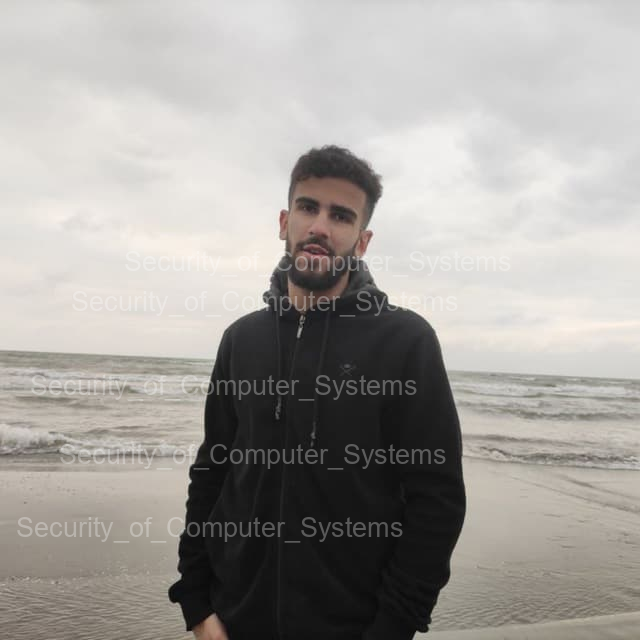
\includegraphics[width=0.7\textwidth]{Images/watermarked.png}
  \caption{تصویر \lr{watermark} شده}   
\end{figure}
سپس تصویر واترمارک شده را تحت چهار عملیات چرخش، برش، تغییر اندازه و افزودن نویز بررسی کردیم. همانطور که مشاهده می‌کنید، واترمارک‌ها از بین نرفته‌اند و نشان‌دهنده‌ی غیرشکننده و قابل مشاهده بودن آن است. 
\begin{figure}[H]
  \centering
  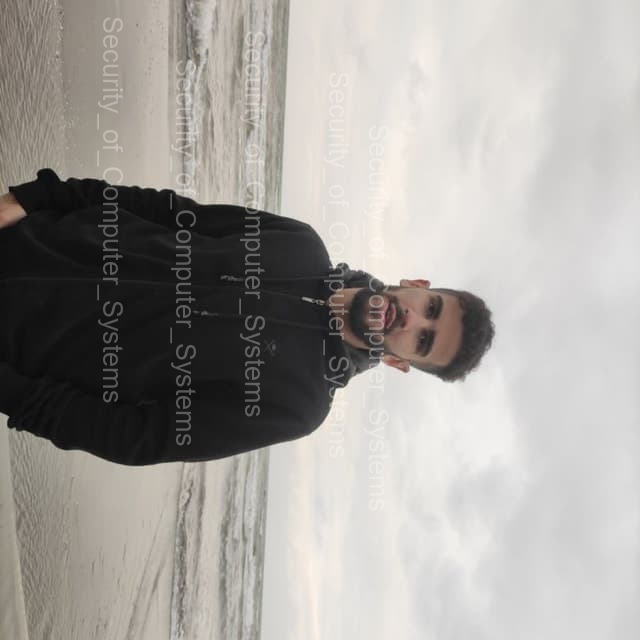
\includegraphics[width=0.7\textwidth]{Images/rotated.png}
  \caption{اعمال چرخش بر روی تصویر \lr{watermark} شده}   
\end{figure}
\begin{figure}[H]
  \centering
  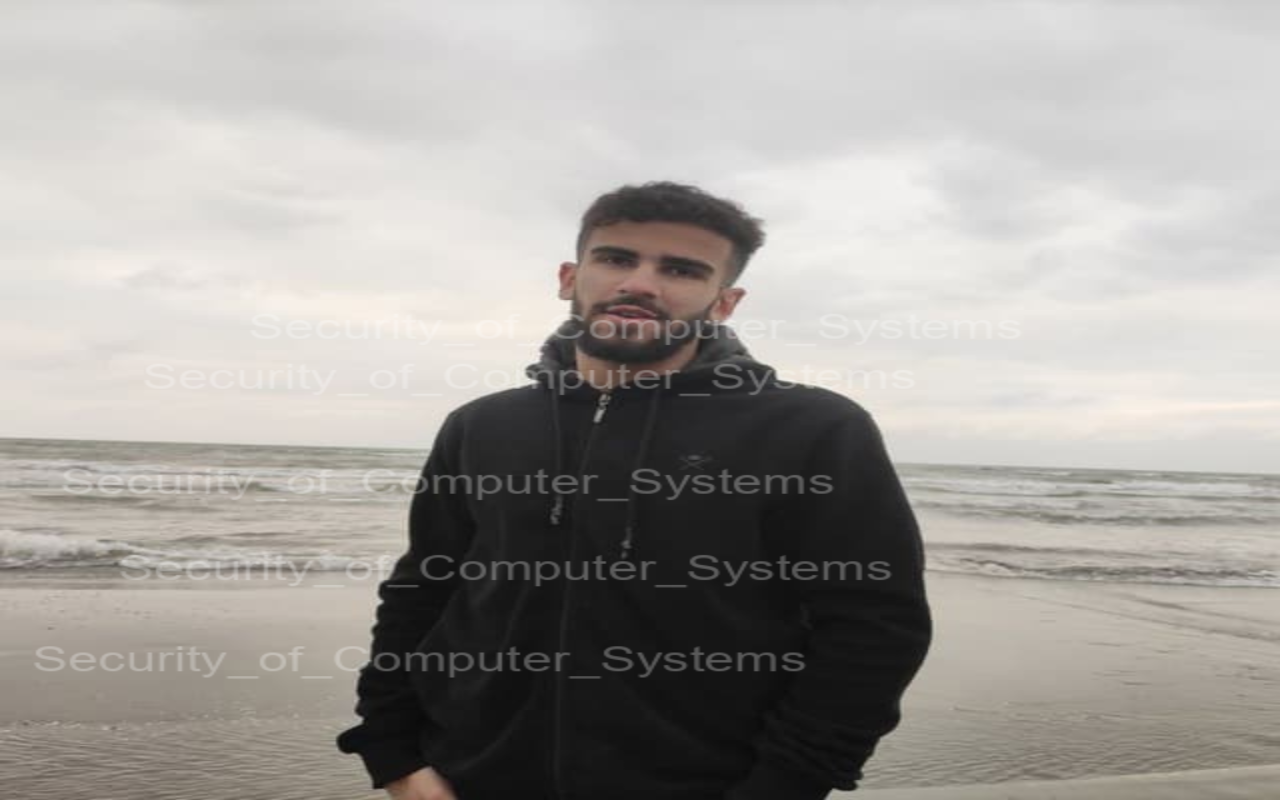
\includegraphics[width=0.7\textwidth]{Images/resized.png}
  \caption{اعمال تغییر اندازه بر روی تصویر \lr{watermark} شده}   
\end{figure}
\begin{figure}[H]
  \centering
  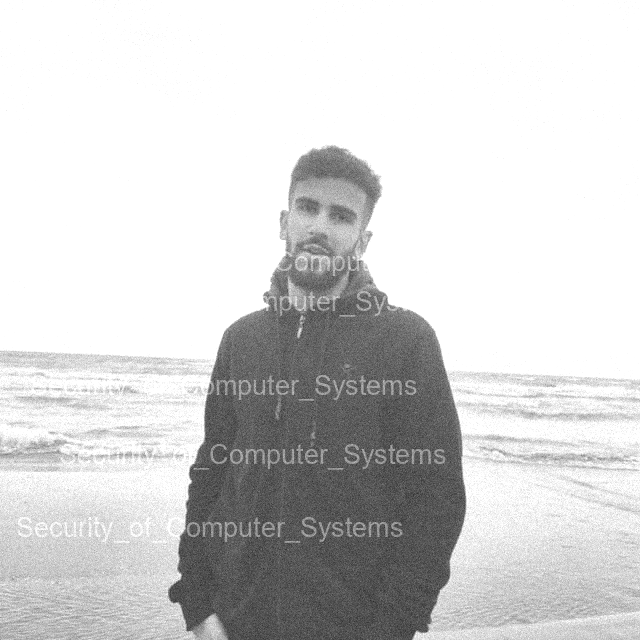
\includegraphics[width=0.7\textwidth]{Images/noisy.png}
  \caption{اعمال نویز بر روی تصویر \lr{watermark} شده}   
\end{figure}
\begin{figure}[H]
  \centering
  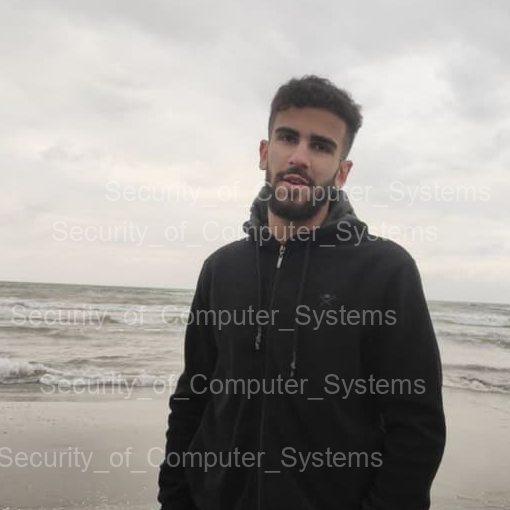
\includegraphics[width=0.7\textwidth]{Images/cropped.png}
  \caption{اعمال برش بر روی تصویر \lr{watermark} شده}   
\end{figure}
\begin{latin}
\href{https://holypython.com/how-to-watermark-images-w-python-pil/}{\textcolor{blue}{Reference}}
\end{latin}

\end{document}